\documentclass{beamer}

% For more themes, color themes and font themes, see:
% http://deic.uab.es/~iblanes/beamer_gallery/index_by_theme.html
%
\mode<presentation>
{
  %\usetheme{Frankfurt}       % or try default, Darmstadt, Warsaw, ...
  %\usetheme{Malmoe}
  \usetheme{Madrid}
  \usecolortheme{default} % or try albatross, beaver, crane, ...
  \usefonttheme{serif}    % or try default, structurebold, ...
  \setbeamertemplate{navigation symbols}{}
  \setbeamertemplate{caption}[numbered]
} 

\usepackage[brazil,portuguese]{babel}
\usepackage[utf8x]{inputenc}
\usepackage{chemfig}
\usepackage[version=3]{mhchem}
\usepackage{wrapfig}

\usepackage{floatflt,graphicx}
% On Overleaf, these lines give you sharper preview images.
% You might want to `comment them out before you export, though.
\usepackage{pgfpages}
\pgfpagesuselayout{resize to}[%
  physical paper width=8in, physical paper height=6in]

\makeatletter
\long\def\beamer@author[#1]#2{%
  \def\insertauthor{\def\inst{\beamer@insttitle}\def\and{\beamer@andtitle}%
  \begin{tabular}{l}#2\end{tabular}}%
  \def\beamer@shortauthor{#1}%
  \ifbeamer@autopdfinfo%
    \def\beamer@andstripped{}%
    \beamer@stripands#1 \and\relax
    {\let\inst=\@gobble\let\thanks=\@gobble\def\and{, }\hypersetup{pdfauthor={\beamer@andstripped}}}
  \fi%
}
\makeatother
\setbeamertemplate{caption}{\raggedright\insertcaption\par}
  
% Here's where the presentation starts, with the info for the title slide
\institute{Universidade Técnológica Federal do Paraná - Campus Pato Branco\\Departamento Acadêmico de Informática\\Curso de Engenharia de Computação}
\title{Consultas por similaridade em bases de dados complexos utilizando técnica OMNI em SGBDR}
\subtitle{Trabalho de Conclusão de Curso}
\author{
Aluno: Cristiano José Mendes Matsui\\
Orientador: Dr. Ives Renê Venturini Pola\\
Coorientadora: Dra. Fernanda Paula Barbosa Pola
}
\date{\today}

\begin{document}


\begin{frame}[plain]
     \vfill
     \centering

     \begin{beamercolorbox}[sep=8pt,center,colsep=-4bp,rounded=true,shadow=true]{institute}
        \usebeamerfont{institute}\insertinstitute
     \end{beamercolorbox}

     {\usebeamercolor[fg]{titlegraphic}\inserttitlegraphic\par}

     \begin{beamercolorbox}[sep=8pt,center,colsep=-4bp,rounded=true,shadow=true]{title}
        \usebeamerfont{title}\inserttitle\par%
        \ifx\insertsubtitle\@empty%
        \else%
        \vskip0.25em%
        {\usebeamerfont{subtitle}\usebeamercolor[fg]{subtitle}\insertsubtitle\par}%
      \fi%     
     \end{beamercolorbox}%

     \vskip1em\par

     \begin{beamercolorbox}[sep=8pt,center,colsep=-4bp,rounded=true,shadow=true]{author}
        \usebeamerfont{author}\insertauthor
     \end{beamercolorbox}

     \begin{beamercolorbox}[sep=8pt,center,colsep=-4bp,rounded=true,shadow=true]{date}
        \usebeamerfont{date}\insertdate
     \end{beamercolorbox}\vskip0.5em

    \end{frame}
\author{Cristiano Matsui}
\institute{UTFPR}
\title{Trabalho de Conclusão de Curso}
% These three lines create an automatically generated table of contents.
\begin{frame}{Sumário}
  \tableofcontents
\end{frame}

\section{Introdução}

\begin{frame}{Introdução}
  \begin{itemize}
    \item Crescimento do uso de dados multimídia
      \begin{itemize}
	\item Imagens, vídeos, áudio...\newline
      \end{itemize}
    \item ``dados comuns'' x ``dados complexos''\newline
	\begin{figure}[H]
			\centering
			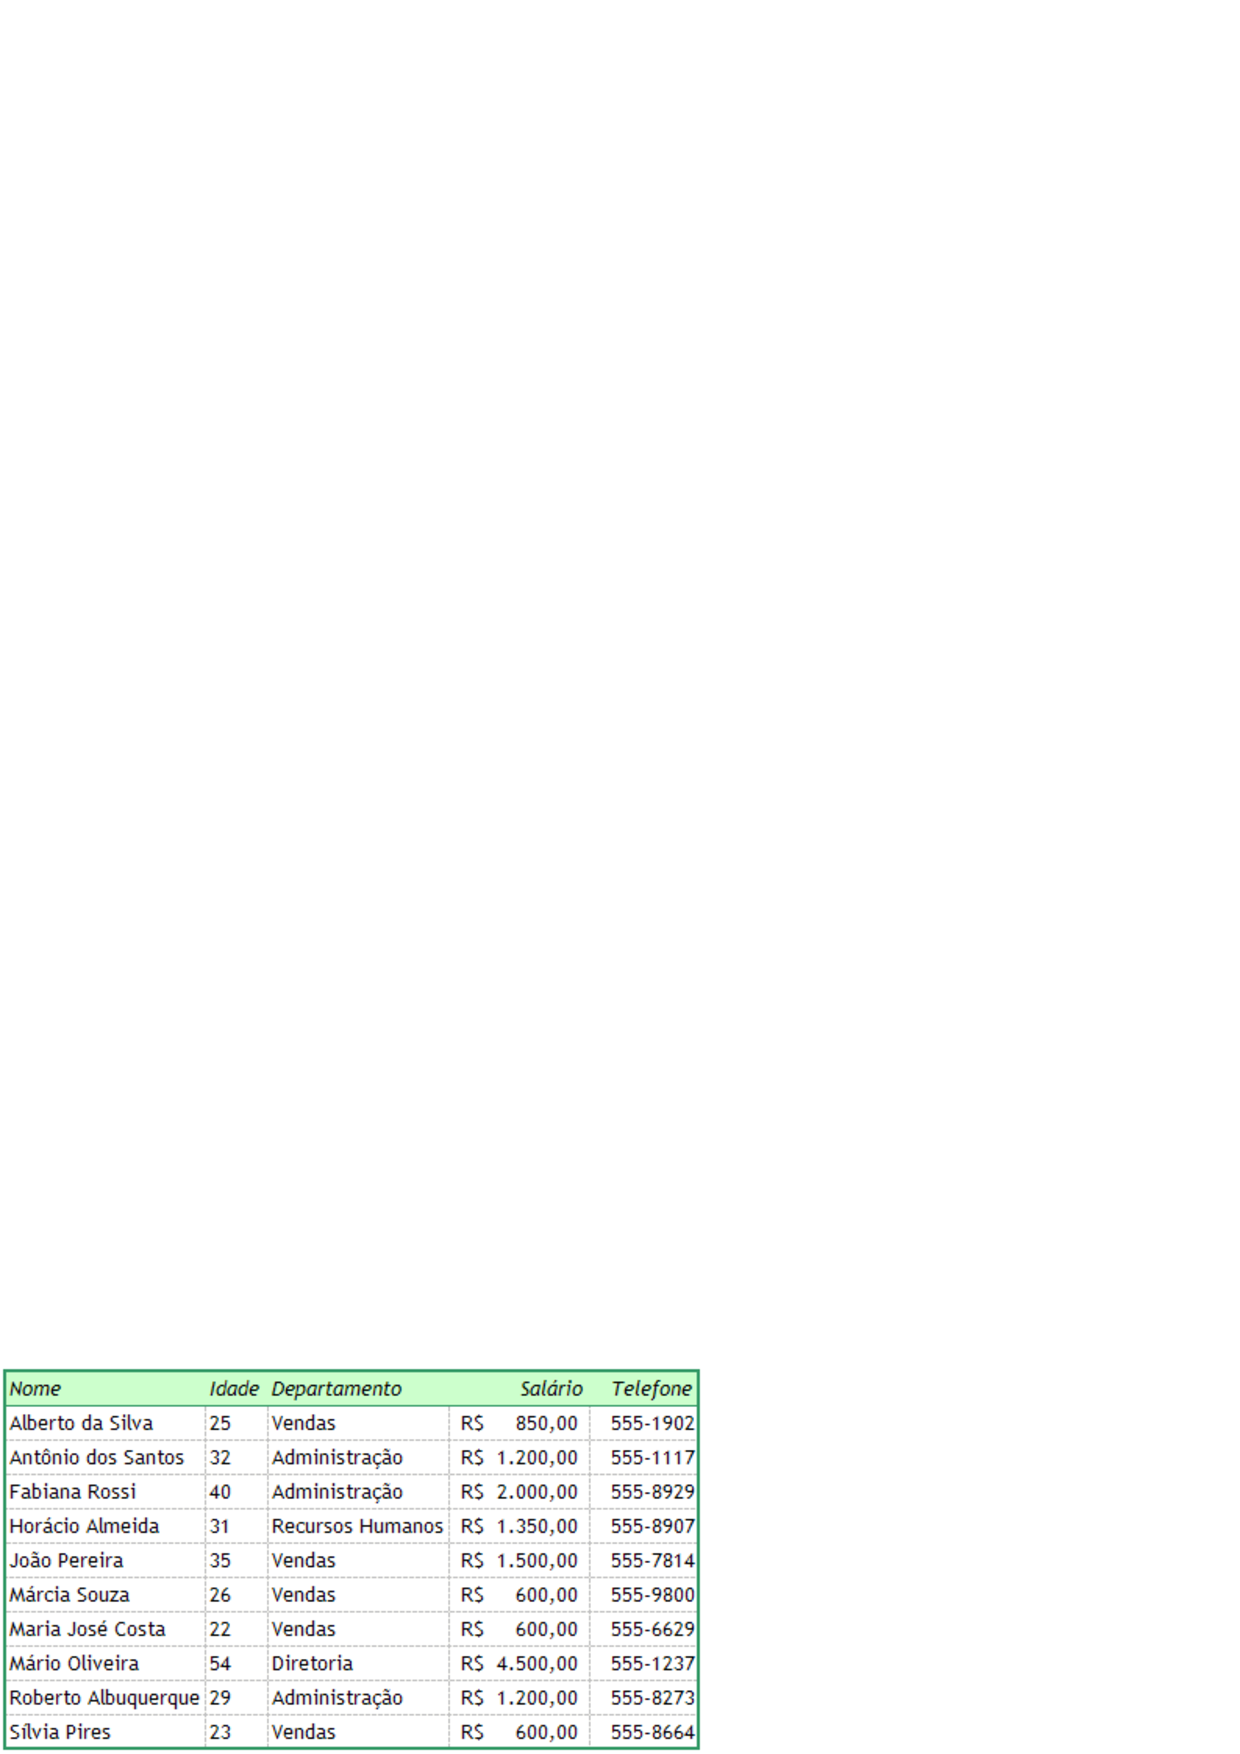
\includegraphics[width=.5\textwidth]{dado_comum.png}
			\label{fig:dado_comum}
	\end{figure}

    \item Problema: consultas com dados complexos\newline
    \item Necessidade de novos operadores de consulta\newline
  \end{itemize}


\end{frame}

\begin{frame}{Introdução}
  \begin{itemize}
   \item Consultas por similaridade\newline
      \begin{itemize}
	  \item Consulta por abrangência(\textit{Range query})\newline
	  \item Consulta aos k-vizinhos mais próximos (\textit{k-Nearest Neighbors query})
      \end{itemize}
	
	\begin{figure}
\centering
\begin{minipage}{.4\textwidth}
  \centering
  \includegraphics[width=.9\linewidth]{rq.png}
  \caption{\textit{Range query}}
  \label{fig:rq}
\end{minipage}%
\begin{minipage}{.6\textwidth}
  \centering
  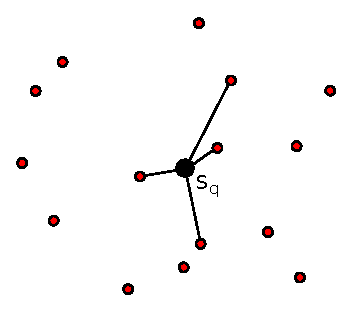
\includegraphics[width=.6\linewidth]{knnq.eps}
  \caption{\textit{kNN query}}
  \label{fig:knnq}
\end{minipage}
\end{figure}
	
  \end{itemize}


\end{frame}

\begin{frame}{Introdução}

  \begin{itemize}
   \item Consultas por similaridade são custosas\newline
   
   \begin{itemize}
      \item Complexidade dos dados\newline
      \item Tamanho da base\newline
   \end{itemize}
   
   \item Torna-se necessário otimizar estes procedimentos\newline
   
   \item Uso da técnica OMNI
  \end{itemize}

 
\end{frame}

\section{Técnica OMNI}

\begin{frame}{Técnica OMNI}

  \begin{itemize}
   \item Reduz o número de cálculos de distância desnecessários\newline
   
   \item Uso de uma base de focos\newline
   
   \item \textit{minimum bounding OMNI region - mbOr}\newline
   
   \item Uso da desigualdade triangular

  \end{itemize}

 
\end{frame}


\begin{frame}{Técnica OMNI}

	\begin{figure}
	    \centering
	    \begin{minipage}{.5\textwidth}
	      \centering
	      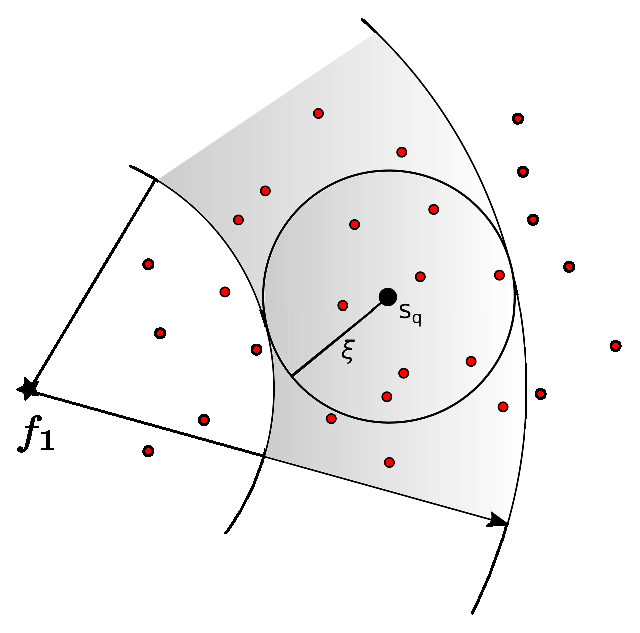
\includegraphics[width=.9\linewidth]{rg_omni_1.eps}


	    \end{minipage}%
	    \begin{minipage}{.5\textwidth}
	      \centering
	      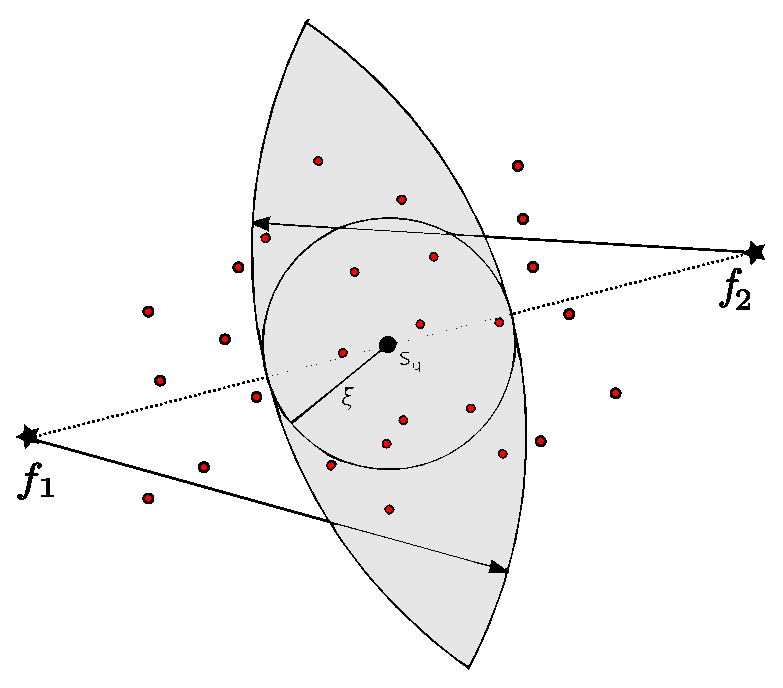
\includegraphics[width=.95\linewidth]{rg_omni_2.eps}


	    \end{minipage}
	\end{figure}
 
\end{frame}

\begin{frame}{Técnica OMNI}
  
  \begin{itemize}
    
   \item Coordenadas OMNI \newline
   
   \item Número de focos
      \begin{itemize}
	\item \textit{Box counting}\newline
	\item ($\lceil D \rceil +1$) \newline
      \end{itemize}
   
    \item Custo do uso da base de focos
      \begin{itemize}
	\item Espaço em disco\newline
	\item Tempo para o cálculo das coordenadas OMNI
      \end{itemize}	
  \end{itemize}

 
\end{frame}

\begin{frame}{Técnica OMNI}	
	\begin{itemize}
	 \item Equação de pertinência à \textit{mbOr}\newline
	    \begin{itemize}
	      \item Desigualdade triangular\newline
		\begin{itemize}
		  \item $d_{f}(s_i) \leq d_{f}(s_q) + d(s_i, s_q)$\newline
		  
		  \item $d(s_i, s_q) \geq |d_{f}(s_i) - d_{f}(s_q)|$\newline
		      \begin{figure}[!H]
			\vspace{-2.5cm}
			\hspace{4cm}
			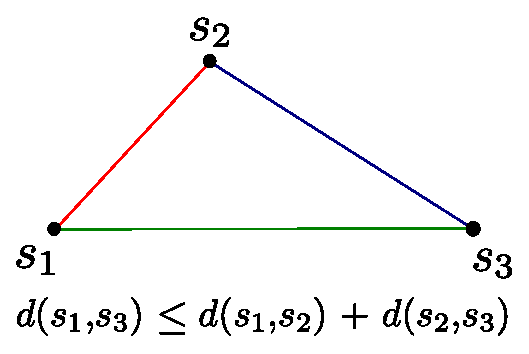
\includegraphics[width=.35\textwidth]{desig_tri.eps}
		      \end{figure}
		\end{itemize}
	      \item Conceito de bola\newline
		\begin{itemize}
		  \item $d(s_i, s_q) \leq \xi$\newline
		\end{itemize}
	    \end{itemize}
	\item $\xi \geq d(s_i,s_q) \geq |d_f(s_i) - d_f(s_q)|$\newline
	\item $|d_f(s_i) - d_f(s_q)| \leq \xi$
	\end{itemize}

\end{frame}

\begin{frame}{Técnica OMNI}
	\begin{itemize}
	 \item $|d_f(s_i) - d_f(s_q)| > \xi$\newline
	 \item Não pertence à \textit{mbOr}!
	\end{itemize}

	\begin{figure}[H]
			\centering
			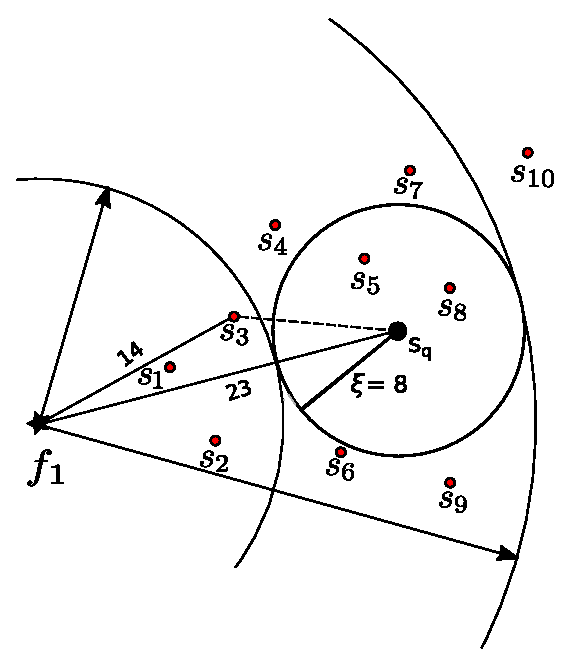
\includegraphics[width=.4\textwidth]{rg_ex2.eps}
	\end{figure}

\end{frame}

\section{Bases de Dados}

\begin{frame}{Bases de Dados}
  \begin{itemize}
   \item Duas bases de dados utilizadas\newline
  \item CAT\_DOG - 25000 imagens
      \begin{itemize}
       \item Imagens de cães e gatos
       \item Cor - Histograma
       \item Textura - dissimilaridade, contraste, correlação
       \item Forma - área, excentricidade, área convexa\newline
      \end{itemize}

  \item HC - 500000 imagens
      \begin{itemize}
	\item Características de imagens médicas já extraídas
	\item Histograma de 256 tons de cinza
      \end{itemize}
      
  \end{itemize}

\end{frame}


\begin{frame}{Extratores de Características}
  \begin{itemize}
   \item Atributos visuais\newline
   \begin{itemize}
      \item Cor
	  \begin{itemize}
	      \item Histograma de cores\newline
	  \end{itemize}
      \item Textura
	  \begin{itemize}
	      \item Descritores de Haralick\newline
	  \end{itemize}
      \item Forma
	  \begin{itemize}
	      \item Análise de contorno\newline
	  \end{itemize}
   \end{itemize}
   
  \end{itemize}

\end{frame}

\begin{frame}{Extratores de Características}
  \begin{itemize}
   \item Histograma de cores
   \begin{itemize}
      \item Discretização e contagem\newline
      \item Computacionalmente simples\newline
      \item Pouca sensibilidade a alterações\newline
      \item Imagens diferentes podem apresentar histogramas de cor parecidos
  \end{itemize} 
 \end{itemize}
	\begin{figure}
\centering
\begin{minipage}{.4\textwidth}
  \centering
  \includegraphics[width=.9\linewidth]{same2.jpg}
\end{minipage}%
\begin{minipage}{.4\textwidth}
  \centering
  \includegraphics[width=.9\linewidth]{histo_same2.png}

\end{minipage}
\end{figure}

\end{frame}

\begin{frame}{Extratores de Características}
  \begin{itemize}
   \item Descritores de Haralick\newline
   \begin{itemize}
      \item Matrizes de co-ocorrência\newline
      \item Análise dos níveis de cinza na imagem\newline
      \item Total de 13 características de textura\newline
	\begin{itemize}
	    \item Contraste, correlação, entropia...\newline
	\end{itemize}
     \item Especialmente útil na área médica
   \end{itemize}
   
  \end{itemize}

\end{frame}

\begin{frame}{Extratores de Características}
  \begin{itemize}
   \item Análise de forma\newline
   \begin{itemize}
      \item Principal análise feita pelo olho humano\newline
      \item Análise de bordas\newline
   \end{itemize}
   
  \end{itemize}
  	\begin{figure}
	    \centering
	    \begin{minipage}{.4\textwidth}
	      \centering
	      \includegraphics[width=.9\linewidth]{onca.jpg}
	    \end{minipage}%
	    \begin{minipage}{.4\textwidth}
	      \centering
	      \includegraphics[width=.9\linewidth]{pantera.jpg}
	    \end{minipage}
\end{figure}

\end{frame}

\section{Modelagem}
\begin{frame}{Modelagem}
    	\begin{figure}[H]
			\centering
			\includegraphics[width=.8\textwidth]{MER.png}
	\end{figure}

\end{frame}

\section{Objetivos}

\begin{frame}{Objetivos}
  \begin{itemize}
   \item Objetivos Gerais
   \begin{itemize}
      \item Construção de um sistema de consultas em SGBDR por similaridade em uma base de imagens utilizando técnicas da família OMNI para reduzir o custo computacional das operações de consulta\newline
   \end{itemize}
   \item Objetivos Específicos
   \begin{itemize}
      \item Modelar o banco de dados para atender a problemática apresentada;
      \item Aplicar os extratores de características das imagens utilizadas;
      \item Inserir no banco de dados as imagens e os valores de suas características;
      \item Criar a estrutura OMNI necessária para a filtragem dos cálculos;
      \item Analisar e comparar os resultados obtidos.
   \end{itemize}
   
  \end{itemize}

\end{frame}

\section{Materiais}

\begin{frame}{Materiais}
  \begin{itemize}
   \item PostgreSQL\newline
   \item Arboretum (GBDI)
   \begin{itemize}
      \item Artemis - Extratores de características
      \item Hermes - Funções de distância\newline
   \end{itemize}
   \item Software para elaboração da interface com o usuário   
  \end{itemize}

\end{frame}



\section{Considerações Finais}

\begin{frame}{Considerações Finais}
  \begin{itemize}
   \item Planeja-se utilizar este trabalho para a elaboração de um CBIR médico\newline
   \begin{itemize}
      \item Suporte para pesquisas por similaridade\newline
         \begin{itemize}
	    \item Totalmente inserido dentro de um SGBDR\newline
	    \item Utilizando técnicas OMNI
	  \end{itemize}
   \end{itemize}
  \end{itemize}
\end{frame}


\institute{Universidade Técnológica Federal do Paraná - Campus Pato Branco\\Departamento Acadêmico de Informática\\Curso de Engenharia de Computação}
\title{Consultas por similaridade em bases de dados complexos utilizando técnica OMNI em SGBDR}
\subtitle{Trabalho de Conclusão de Curso}
\author{
Aluno: Cristiano Matsui\\
Orientador: Dr. Ives Renê Venturini Pola\\
Coorientadora: Dra. Fernanda Paula Barbosa Pola
}
\date{\today}



\begin{frame}[plain]
     \vfill
     \centering

     \begin{beamercolorbox}[sep=8pt,center,colsep=-4bp,rounded=true,shadow=true]{institute}
        \usebeamerfont{institute}\insertinstitute
     \end{beamercolorbox}

     {\usebeamercolor[fg]{titlegraphic}\inserttitlegraphic\par}

     \begin{beamercolorbox}[sep=8pt,center,colsep=-4bp,rounded=true,shadow=true]{title}
        \usebeamerfont{title}\inserttitle\par%
        \ifx\insertsubtitle\@empty%
        \else%
        \vskip0.25em%
        {\usebeamerfont{subtitle}\usebeamercolor[fg]{subtitle}\insertsubtitle\par}%
      \fi%     
     \end{beamercolorbox}%

     \vskip1em\par

     \begin{beamercolorbox}[sep=8pt,center,colsep=-4bp,rounded=true,shadow=true]{author}
        \usebeamerfont{author}\insertauthor
     \end{beamercolorbox}

     \begin{beamercolorbox}[sep=8pt,center,colsep=-4bp,rounded=true,shadow=true]{date}
        \usebeamerfont{date}\insertdate
     \end{beamercolorbox}\vskip0.5em

    \end{frame}

\end{document}